\documentclass[11pt]{article}

\usepackage[margin=1in]{geometry}
\usepackage{graphicx}
\usepackage{booktabs}
\usepackage{amsmath,amssymb}
\usepackage[numbers,sort&compress]{natbib}
\usepackage{hyperref}
\usepackage{url}
\usepackage{microtype}
\usepackage{xcolor}
\usepackage{caption}
\usepackage{array}
\captionsetup{font=small,labelfont=bf}

\title{Chronic activation of a negative memory engram in ventral CA1 induces age-dependent anxiety, cognitive, and glial abnormalities in mice}

\author{}
\date{}

\begin{document}

\maketitle

\begin{abstract}
Chronic stress and repetitive negative thinking are leading risk factors for mood and memory disorders, yet it is unclear whether the repeated reactivation of a negatively valenced memory ensemble is, on its own, sufficient to produce stress-like cellular and behavioral pathology. Existing engram studies have demonstrated that acute reactivation of a tagged ensemble can drive episodic memory expression, but they have not tested the consequences of sustained, month-scale reactivation. We addressed this gap by combining activity-dependent genetic tagging in TRAP2 mice with excitatory chemogenetics (hM3Dq) and chronic, low-dose deschloroclozapine (DCZ) delivered in home-cage drinking water at $3\,\mu\mathrm{g}\,\mathrm{kg}^{-1}\,\mathrm{day}^{-1}$. After tagging a fear-conditioned negative engram in ventral CA1, we reactivated it continuously for three months in young (3-month) and aged (11-month) cohorts that reached 6 and 14 months at endpoint, and assayed anxiety, spatial working memory, fear recall, extinction, and generalization together with hippocampal microglia and astrocyte counts and morphology. Engram transcriptomics indicated that negative (foot shock) and positive (male-to-female exposure) ensembles are biased toward pro- and anti-inflammatory gene programs, respectively. In vivo, chronic engram reactivation increased anxiety-like behavior in the open field (Group $F(1,33)=29.56$, $p<0.0001$) and zero maze (Group $F(1,38)=40.22$, $p<0.0001$) at both ages, reduced Y-maze spontaneous alternation selectively in 14-month mice (Tukey $p=0.0045$), impaired fear extinction in 6-month mice (Group $F(1,17)=5.494$, $p=0.0315$), increased generalization freezing at both ages (Group $F(1,41)=26.53$, $p<0.0001$), and expanded hippocampal Iba1$^{+}$ microglia at 14 months (Tukey $p=0.0113$) and GFAP$^{+}$ astrocytes at both ages ($p=0.0328$ and $p=0.0208$), without reducing NeuN$^{+}$ counts in subiculum, ventral dentate gyrus, or ventral CA1. Together, chronic reactivation of a single negative ventral-CA1 engram is sufficient to induce enduring, age-dependent cellular and behavioral abnormalities that mirror key features of chronic stress and rumination-like states, and provides a causal framework within which to interpret the epidemiological link between repetitive negative thinking and adverse brain outcomes.
\end{abstract}

% =====================================================================
\section{Introduction}

Chronic stress is a leading environmental risk factor for neuropsychiatric disease and contributes to the onset and progression of major depressive disorder, generalized anxiety disorder, and post-traumatic stress disorder. Its cognitive correlate, repetitive negative thinking, is itself prospectively associated with accelerated cognitive decline and with in vivo markers of amyloid and tau accumulation in older adults \citep{marchant2020rnt}. This convergence of a modifiable cognitive process with the biological hallmarks of neurodegeneration raises a causal question that animal models are well placed to answer: does the persistent reactivation of negatively valenced memory representations itself drive downstream cellular and behavioral pathology, or does it simply co-occur with stress-induced changes arising through other routes? Addressing this question requires a model in which a specific, experimentally defined negative memory can be reactivated on demand over long timescales, while cellular and behavioral consequences are measured in a controlled fashion.

The ventral hippocampus, and specifically the ventral CA1 (vCA1) subregion, is a compelling target for such a model. The ventral hippocampus is functionally dissociable from its dorsal counterpart, with ventral subfields aligning with emotion and stress circuitry rather than with purely spatial or cognitive processing \citep{fanselow2010ventral}. Projections from vCA1 to the basolateral amygdala, nucleus accumbens, and medial prefrontal cortex are organized into largely segregated populations that route distinct behaviorally contingent signals to each target, with anxiety-related firing preferentially enriched in prefrontal-projecting neurons \citep{ciocchi2015vca1}. These anatomical and physiological properties place vCA1 in a privileged position to link a learned aversive experience to enduring shifts in affect, vigilance, and context-dependent behavior.

Activity-dependent tagging methods now make it possible to identify, label, and causally manipulate the sparse ensembles that encode specific memories. Optogenetic reactivation of dentate-gyrus neurons active during fear conditioning is sufficient to elicit freezing in a neutral context \citep{liu2012engram}, and the behavioral valence of a hippocampal contextual memory engram is malleable, such that re-pairing reactivation with a stimulus of opposite sign reverses the learned response \citep{redondo2014valence}. Conversely, chronic optogenetic reactivation of dentate cells tagged during a positive experience can rescue stress-induced depressive-like phenotypes \citep{ramirez2015positive}. These findings position engrams as both necessary and sufficient substrates of memory expression \citep{josselyn2020engram}. The complementary possibility---that sustained activation of a negative engram over months is itself sufficient to produce stress-like neural and behavioral pathology, rather than merely to evoke episodic fear expression---has remained largely untested.

Any causal test of this hypothesis must also contend with the well-documented age-dependence of stress vulnerability. Large cross-national surveys show that childhood adversities account for a substantial share of first-onset psychiatric disorders, with effects that persist across the life-course \citep{kessler2010childhood}. The glucocorticoid cascade hypothesis holds that sustained exposure to glucocorticoids progressively compromises hippocampal function \citep{sapolsky1986glucocorticoid}, and adult hippocampal neurogenesis, a substrate for stress resilience, declines steeply with age \citep{klempin2007neurogenesis}. Whether an identical chronic engram-activation protocol produces comparable phenotypes in younger and older animals, or whether age modulates the behavioral and glial consequences, therefore has direct implications for how stress-related disorders should be interpreted across the lifespan.

Here we combine the TRAP2 activity-dependent tagging system \citep{denardo2019temporal} with the high-affinity, metabolically stable muscarinic DREADD actuator deschloroclozapine \citep{nagai2020dcz,roth2016dreadds} to drive chronic reactivation of a fear-conditioned vCA1 engram for three continuous months. We run the protocol in parallel cohorts that begin at 3 months and 11 months of age so that endpoint assays at 6 and 14 months isolate age-dependent differences in the response to an otherwise identical manipulation. We ask whether chronic negative-engram activation is sufficient to induce anxiety-like behavior, spatial working-memory deficits, impaired fear extinction, and enhanced fear generalization \citep{maren2013contextual,tovote2015circuits}, together with microglial and astrocytic remodeling in hippocampus, without overt neuronal loss.

\paragraph{Contributions.} The present study makes four contributions. First, we establish a three-month chronic chemogenetic protocol in which a vCA1 TRAP2-tagged negative engram is reactivated by low-dose DCZ delivered in drinking water, and show that the protocol is well tolerated (normal weight gain across both age groups; no decrease in NeuN$^{+}$ counts in subiculum, ventral dentate gyrus, or vCA1). Second, we demonstrate that chronic negative-engram activation is sufficient to increase anxiety-like behavior in both young and aged mice, as indexed by decreased center time in the open field and decreased open-arm time in the zero maze. Third, we show that the cognitive phenotypes are age-dependent: spatial working memory is selectively impaired at 14 months, fear extinction is selectively impaired at 6 months, and fear generalization to a novel context is enhanced at both ages. Fourth, we show that chronic engram activation remodels hippocampal glia, with age-dependent microglial expansion at 14 months and astrocytic expansion with branch-length elongation at both ages.

% =====================================================================
\section{Related work}

\paragraph{Engram tagging and causal manipulation of memory.}
The operational idea that a specific memory is supported by a sparse, identifiable neural ensemble has been repeatedly validated in rodents using activity-dependent promoters combined with optogenetic or chemogenetic effectors. Optogenetic reactivation of dentate-gyrus cells tagged during fear conditioning is sufficient to evoke freezing in a neutral context \citep{liu2012engram}, and the behavioral valence of an engram can be switched by pairing its reactivation with a stimulus of opposite sign \citep{redondo2014valence}. Reactivation of positive-experience engrams can rescue stress-induced depressive-like phenotypes \citep{ramirez2015positive}, and broader synthesis work has consolidated these findings into a framework in which engrams are the basic functional unit of memory \citep{josselyn2020engram}. Most prior engram-manipulation studies rely on acute or short-term reactivation on the scale of hours to days; the present work extends the manipulation to three continuous months and focuses specifically on the consequences of reactivating an aversive ensemble in vCA1.

\paragraph{Chemogenetic and TRAP2 tools.}
Activity-dependent tagging via targeted recombination in active populations (TRAP2) exploits the cFos promoter together with tamoxifen-gated CreER to capture ensembles active during a defined temporal window, and has been used to track and manipulate fear-related ensembles over time \citep{denardo2019temporal}. DREADDs, particularly the excitatory hM3Dq receptor, have become standard tools for neuronal manipulation because of their reversibility and cell-type specificity \citep{roth2016dreadds}. However, the canonical agonist clozapine-N-oxide has sluggish kinetics and potential off-target liabilities, motivating the development of deschloroclozapine, a high-affinity, selective, fast-acting actuator that drives hM3Dq-mediated activation in rodents and non-human primates at doses of $1$--$3\,\mu\mathrm{g}\,\mathrm{kg}^{-1}$ \citep{nagai2020dcz}. Our low-dose DCZ-in-water protocol builds on this pharmacology but introduces chronic, low-intensity dosing to mimic sustained dysregulation rather than acute, high-amplitude activation.

\paragraph{Ventral hippocampus in affect, stress, and aging.}
The ventral hippocampus is the hippocampal subfield most closely linked to emotional processing, stress reactivity, and affective disease \citep{fanselow2010ventral}. Recordings during anxiety-related behavior show that subsets of vCA1 projection neurons preferentially route anxiety- or reward-related information to prefrontal cortex, nucleus accumbens, or amygdala \citep{ciocchi2015vca1}. At the systems level, childhood adversity confers lifelong, cross-diagnostic risk for psychopathology \citep{kessler2010childhood}, consistent with the glucocorticoid cascade model in which repeated stress progressively degrades hippocampal function \citep{sapolsky1986glucocorticoid} and with the decline of adult hippocampal neurogenesis over the lifespan \citep{klempin2007neurogenesis}. Our design addresses the age dimension directly by running an identical chemogenetic protocol in cohorts that reach 6 and 14 months at endpoint.

\paragraph{Fear circuitry, extinction, and generalization.}
Fear memory, extinction, and generalization are supported by a hippocampus-amygdala-medial-prefrontal network in which context integration is especially dependent on the hippocampus \citep{maren2013contextual,tovote2015circuits}. Impaired extinction and overgeneralization of fear to non-threatening contexts are core phenotypes in anxiety and PTSD models. Our extinction and Context~B generalization assays use this framework to ask whether chronic reactivation of a vCA1 negative engram produces deficits that mirror human anxiety-spectrum pathology.

% =====================================================================
\section{Methods}

\subsection{Animals}
TRAP2 mice were used for all experiments, with two cohorts that were 3 months and 11 months old at the time of surgery, so that the endpoint assays (after 3 months of chronic stimulation) were performed at 6 and 14 months, respectively. After surgery, mice were group-housed with littermates and allowed to recover for a minimum of 4 weeks prior to experimentation to allow for viral expression. All procedures were conducted under protocol 201800579 approved by the Institutional Animal Care and Use Committee at Boston University.

\subsection{Stereotaxic surgery}
Mice were anesthetized with 3.0\% isoflurane during induction and maintained at 1--2\% through a stereotaxic nose cone (oxygen 1\,L\,min$^{-1}$). The scalp was depilated with a commercial hair-removal cream and cleaned with alternating applications of betadine and 70\% ethanol. Lidocaine hydrochloride (2.0\%) was injected subcutaneously as local analgesia prior to a midsagittal incision, and meloxicam ($0.1\,\mathrm{mg\,kg^{-1}}$ at $5\,\mathrm{mg\,kg^{-1}}$ stock) was administered subcutaneously at the beginning of surgery. Bilateral craniotomies ($0.5$--$0.6\,\mathrm{mm}$ drill) were made over vCA1. A 10-$\mu$L airtight Hamilton syringe with a 33-gauge beveled needle was lowered to coordinates $-3.16$\,AP, $\pm 3.10$\,ML, and $-4.25$/$-4.50$\,DV relative to bregma to cover the vertical axis of ventral hippocampus. A total volume of 300\,nL of AAV9-DIO-Flex-hM3Dq-mCherry or AAV9-DIO-Flex-mCherry was injected bilaterally into vCA1, split as 150\,nL at each DV depth. Following surgery, mice received $0.1\,\mathrm{mg\,kg^{-1}}$ buprenorphine intraperitoneally. Histological assessment verified bilateral viral targeting, and data from off-target injections were excluded.

\subsection{Negative engram tagging}
After a recovery period of at least two weeks, mice were subjected to contextual fear conditioning (CFC), consisting of four $1.5\,\mathrm{mA}$ foot shocks in Context~A. Thirty minutes after CFC, mice received a $40\,\mathrm{mg\,kg^{-1}}$ intraperitoneal injection of 4-hydroxytamoxifen (4-OHT) to label cells sufficiently active during the fearful experience, consistent with the canonical TRAP2 paradigm \citep{denardo2019temporal}.

\subsection{Chronic DCZ administration}
Home-cage water was replaced with water-soluble deschloroclozapine dihydrochloride in distilled water every 5 days \citep{nagai2020dcz,roth2016dreadds}. A stock solution was prepared by dissolving 1--2\,mg of DCZ in 1\,mL of DMSO; 17\,$\mu$L of stock solution was combined with 1\,L of distilled water for a final concentration designed to deliver $3\,\mu\mathrm{g}\,\mathrm{kg}^{-1}\,\mathrm{day}^{-1}$ assuming $\sim\!6\,\mathrm{mL}$ per-mouse daily intake. When administered intraperitoneally in mice, DCZ plasma levels peak 5--10 min after injection and decline to baseline around 2 h post-injection; the drinking-water route was chosen to convert this short-lived high-amplitude pharmacokinetic profile into a sustained, low-amplitude exposure over months. This low-dose, constant dosing regimen was also chosen to avoid potential excitotoxicity during up to three continuous months of stimulation and to mimic sustained dysregulation that may accumulate in severity over time. No signs of distress or seizures were observed during the entire chronic-administration window.

\subsection{Behavioral battery}
After three months of DCZ-mediated hM3Dq activation, all mice underwent a matched battery of assays. The open field was a $61\,\mathrm{cm}\times 61\,\mathrm{cm}$ arena with black plastic walls and a red-taped center region, in which mice explored freely for 10\,min. The zero maze consisted of a $44\,\mathrm{cm}$-wide ring with an outer diameter of $62\,\mathrm{cm}$, $8\,\mathrm{cm}$ in height, elevated $66\,\mathrm{cm}$ off the ground. The Y-maze comprised three clear plexiglass arms ($36.5\,\mathrm{cm}$ length, $7.5\,\mathrm{cm}$ width, $12.5\,\mathrm{cm}$ height) intersecting at $120^{\circ}$. Remote recall and extinction sessions returned mice to Context~A (a $18.5\,\mathrm{cm}\times 18.5\,\mathrm{cm}\times 21.5\,\mathrm{cm}$ chamber with metal walls, plexiglass front and back, and a 16-bar stainless-steel grid floor) for 5\,min and 30\,min, respectively, in the absence of foot shocks. Generalization was assessed in a novel, larger chamber (Context~B) in a different room. Chambers and mazes were cleaned with 70\% ethanol between animals. Mice were handled for 2\,min per day for 3--5 days before behavior.

\subsection{Immunohistochemistry and morphology}
Mice were deeply anesthetized with 3\% isoflurane and perfused transcardially with cold PBS followed by 4\% paraformaldehyde. Brains were post-fixed in PFA at $4\,^{\circ}\mathrm{C}$ for 24--48\,h, transferred to 30\% sucrose/PBS, and stored in 0.01\% sodium azide/PBS. Coronal and sagittal sections (50\,$\mu$m) were cut on a vibratome. Sections were blocked in PBST with 5\% normal goat serum for 2\,h at room temperature. NeuN z-stacks were acquired at 4\,$\mu$m intervals, whereas Iba1 and GFAP z-stacks were acquired at 1\,$\mu$m intervals for detailed morphological analysis. Glial morphology was quantified using 3DMorph, a MATLAB-based toolbox for three-dimensional microglial and astrocytic morphometry \citep{york2018threedmorph}. For cell counts, $n=3$ mice per group $\times$ 18 single-tile ROIs per region (NeuN, GFAP, Iba1). For morphology, $n=3$ mice per group $\times$ 3 ROIs per field, with 20--30 glial cells each.

\subsection{Transcriptomics and GSEA}
For engram transcriptomics, tagged positive (male-to-female exposure) and negative (foot shock) engram cells were isolated via MACS SmartStrainers (70\,$\mu$m). RNA-seq libraries were prepared with the SMART-Seq v4 Ultra Low Input RNA Kit (TaKaRa Bio). Gene-level fold changes were used to rank protein-coding genes, and the GseaPreranked tool was used for pathway enrichment analysis.

\subsection{Statistics}
Data were analyzed in GraphPad Prism v9.4.1. Two-way (RM) ANOVAs were followed by Sidak's or Tukey's post-hoc tests, as indicated throughout. Outliers were identified using ROUT with $Q=10\%$. Sample sizes were $n=9$--$17$ per group after outlier removal for behavioral assays and $n=3$ mice per group for histology. Significance thresholds throughout are $p \leq 0.05$ (*), $p \leq 0.01$ (**), $p \leq 0.001$ (***), $p \leq 0.0001$ (****); ``ns'' denotes not significant.

% =====================================================================
\section{Results}

\subsection{Transcriptional signatures distinguish positive and negative memory engrams}

We first asked whether positive and negative memory engrams exhibit distinct molecular signatures that could predispose them to different downstream consequences upon repeated reactivation. To address this question, we isolated TRAP2-tagged engram cells corresponding to a positive experience (male-to-female exposure) and a negative experience (foot-shock fear conditioning), prepared SMART-Seq v4 Ultra Low Input RNA-seq libraries, and ranked protein-coding genes by fold change for pre-ranked Gene Set Enrichment Analysis.

The GSEA output revealed a striking valence-specific transcriptional signature: cells carrying a positive engram were enriched for anti-inflammatory gene programs, whereas cells carrying a negative engram were enriched for pro-inflammatory gene programs. Because the pre-ranked GSEA uses the full fold-change distribution of protein-coding genes rather than a hard-thresholded hit list, this contrast represents a genome-wide bias of the two ensembles rather than a handful of individually significant genes, and is therefore a candidate substrate for longer-timescale physiological divergence. This molecular dissociation suggests that the long-term biological consequences of reactivating these two ensembles may also diverge, with negative engrams biased toward inflammation-linked outcomes. That observation motivated us to ask whether chronic in vivo reactivation of the negative engram, beyond its acute effects on fear recall, could produce enduring cellular and behavioral changes in the hippocampus, and whether those changes would depend on the age at which the manipulation was delivered.

\subsection{Chronic chemogenetic reactivation of a vCA1 negative engram does not disrupt body weight or neuronal counts}

To test whether a sustained reactivation of the vCA1 negative engram is tolerated in vivo, we combined three well-validated components: the TRAP2 line for activity-dependent tagging \citep{denardo2019temporal}, the excitatory DREADD hM3Dq \citep{roth2016dreadds}, and the high-affinity actuator deschloroclozapine delivered in drinking water at a sustained low dose \citep{nagai2020dcz}. TRAP2 mice received bilateral vCA1 injections of AAV9-DIO-Flex-hM3Dq-mCherry or AAV9-DIO-Flex-mCherry, underwent contextual fear conditioning (four $1.5\,\mathrm{mA}$ foot shocks) paired with $40\,\mathrm{mg\,kg^{-1}}$ 4-OHT to tag the negative engram, and were then placed on DCZ drinking water ($3\,\mu\mathrm{g\,kg^{-1}\,day^{-1}}$, refreshed every 5 days) for three months (Figure~\ref{fig:design}).

Body weight of both young (6-month endpoint) and aged (14-month endpoint) mice increased over the three-month stimulation period, as expected from normal age-related weight gain, without any effect of hM3Dq activation. Two-way repeated-measures ANOVAs revealed a main effect of Month in both cohorts (6-month: $F(2,34)=14.84$, $p<0.0001$; 14-month: $F(2,52)=7.854$, $p=0.0010$) but no significant Group effect (6-month: $F(1,17)=1.361$, $p=0.2594$; 14-month: $F(1,26)=0.1275$, $p=0.7239$) and no Month-by-Group interaction (6-month $p=0.7701$; 14-month $p=0.0833$). Sidak's post-hoc tests confirmed the expected monotonic weight increase across months (e.g., 6-month 1~vs.~3, $p<0.0001$; 14-month 1~vs.~3, $p=0.0011$). We note that body weight was first measured at Month~1 rather than at baseline, leaving open the possibility of an early, transient drop during Month~0--1 that rebounded before our first measurement.

We next asked whether three months of chronic vCA1 activation produced detectable neuronal loss. Stereological NeuN$^{+}$ counts in subiculum, ventral dentate gyrus (vDG), and ventral CA1 (vCA1) were indistinguishable between hM3Dq and age-matched mCherry controls (subiculum Group $F(1,8)=0.00721$, $p=0.9344$; vDG Group $F(1,8)=0.0524$, $p=0.8246$; vCA1 Group $F(1,8)=2.947$, $p=0.1244$; Figure~\ref{fig:neun}). Tukey's post-hoc comparisons on the subiculum data yielded 6MO mCherry vs.~hM3Dq $p=0.9904$ and 14MO mCherry vs.~hM3Dq $p=0.9744$. These data indicate that, despite months of sustained chemogenetic activation, the protocol does not reduce the density of NeuN$^{+}$ neurons in the core regions targeted. Having established that the chronic protocol is physiologically tolerated, we next examined whether it produced behavioral abnormalities.

\subsection{Chronic negative-engram activation increases anxiety-like behavior at both ages}

To test whether chronic activation of a negative engram is sufficient to increase anxiety-like behavior, we ran the open field and zero maze assays three months into stimulation (Figure~\ref{fig:behavior}). In the open field, 6- and 14-month hM3Dq mice spent less time in the center than age-matched mCherry controls, with a strong and unambiguous Group main effect (Two-way ANOVA Group $F(1,33)=29.56$, $p<0.0001$; Tukey 6MO mCherry vs.~hM3Dq $p=0.0049$; 14MO mCherry vs.~hM3Dq $p=0.0016$). There was no main effect of Age ($F(1,33)=0.5858$, $p=0.4495$) and no Age-by-Group interaction ($p=0.7070$), indicating that the anxiogenic effect of chronic engram activation was comparable in the two cohorts.

Importantly, this decrease in center time was not explained by gross differences in locomotion. Total distance traveled did not differ across groups (Interaction $F(1,37)=0.0016$, $p=0.9675$; Age $F(1,37)=0.6862$, $p=0.4128$; Group $F(1,37)=0.3522$, $p=0.5565$), nor did the number of center entries (Interaction $F(1,41)=1.236$, $p=0.2728$; Group $F(1,41)=0.3370$, $p=0.5648$), implying that hM3Dq mice visited the center as often as controls but spent less time per visit. Six-month hM3Dq mice did, however, show increased average speed in the open field (Group $F(1,38)=7.306$, $p=0.0102$; Tukey 6MO mCherry vs.~hM3Dq $p=0.0150$; 14MO mCherry vs.~hM3Dq $p=0.9532$), consistent with an agitation-like rather than suppression-of-movement phenotype.

The zero-maze results reinforced this interpretation. Both 6- and 14-month hM3Dq mice spent less time in the open arms than age-matched mCherry mice (Group $F(1,38)=40.22$, $p<0.0001$; Tukey 6MO $p=0.0002$; 14MO $p=0.0007$; Figure~\ref{fig:behavior}). As in the open field, there were no group differences in total distance traveled (Group $F(1,36)=0.6022$, $p=0.4428$), open-area entries (Group $F(1,38)=3.286$, $p=0.0778$), or average speed (Group $F(1,37)=0.7180$, $p=0.4023$), indicating that the avoidance of the exposed open arms reflects an anxiety-like bias rather than general hypoactivity. Figure~\ref{fig:age_by_group} further shows that the Group effects were robust at both ages for both assays.

\subsection{Chronic negative-engram activation impairs spatial working memory selectively in aged mice}

We then asked whether chronic negative-engram activation also perturbs spatial working memory, using spontaneous alternation in the Y-maze as an index. Here the two age groups diverged. A two-way ANOVA revealed a significant Age-by-Group interaction ($F(1,40)=4.088$, $p=0.0499$) and a Group main effect ($F(1,40)=7.517$, $p=0.0091$). Tukey's post-hoc comparisons localized the effect to the aged cohort: 14-month hM3Dq mice had a reduced percentage of spontaneous alternations compared with 14-month mCherry mice ($p=0.0045$), whereas 6-month hM3Dq and mCherry mice were statistically indistinguishable ($p=0.9634$; Figure~\ref{fig:age_by_group}).

This selective vulnerability was not an artifact of gross motor or motivation differences: total distance traveled in the Y-maze did not differ between groups (Interaction $F(1,44)=0.2668$, $p=0.6081$; Group $F(1,44)=1.181$, $p=0.2831$), nor did total arm entries (Interaction $F(1,40)=1.332$, $p=0.2553$; Group $F(1,40)=0.8247$, $p=0.3692$). The finding that aged, but not young, hM3Dq mice show reduced alternation is consistent with the broader notion that the aged brain is more vulnerable to chronic stress-like perturbations of hippocampus-dependent function \citep{sapolsky1986glucocorticoid,klempin2007neurogenesis}. It also contrasts with the fear-extinction profile described in the next section, highlighting that different age groups express different cognitive costs of the same chronic manipulation.

\subsection{Chronic negative-engram activation impairs fear extinction in young mice and increases fear generalization at both ages}

To ask whether chronic engram activation perturbs fear memory dynamics rather than just novel-environment behavior, we measured remote recall, extinction, and generalization. During the initial 300-s CFC session, freezing behavior did not differ between mCherry and hM3Dq mice in either cohort (6MO Group $F(1,26)=2.737$, $p=0.1101$; 14MO Group $F(1,18)=1.862$, $p=0.1892$), confirming that the chronic manipulation did not distort the formation of the initial fear association. Three months later, in a remote recall test in Context~A, 6-month hM3Dq mice froze more than 6-month mCherry mice (Group $F(1,17)=6.588$, $p=0.0200$; Tukey 6MO mCherry vs.~hM3Dq $p=0.0449$), whereas 14-month cohorts did not differ at the Group level ($F(1,26)=0.3967$, $p=0.5343$). Independent of the chemogenetic manipulation, 14-month mCherry mice froze more than 6-month mCherry mice (Tukey 6 vs.~14MO mCherry $p=0.0101$), consistent with previously reported age effects on fear recall.

Extinction (a 30-min session in Context~A in the absence of foot shocks) revealed a similar pattern of age-specific vulnerability. Six-month hM3Dq mice maintained elevated freezing relative to 6-month mCherry mice (Group $F(1,17)=5.494$, $p=0.0315$), whereas 14-month cohorts did not differ at the Group level ($F(1,26)=0.3836$, $p=0.5411$). These data indicate that chronic engram activation specifically impaired the ability of young mice to reduce fear expression over an extended non-reinforced exposure---an extinction-resistance phenotype that parallels a core deficit of human anxiety disorders \citep{maren2013contextual,tovote2015circuits}.

In the novel Context~B used to assess generalization, both age groups of hM3Dq mice froze more than age-matched mCherry controls (Group $F(1,41)=26.53$, $p<0.0001$; Tukey 6MO $p=0.0053$; 14MO $p=0.0026$; Figure~\ref{fig:behavior}). The Context~B result indicates that chronic reactivation of a negative engram broadens the range of contexts that elicit defensive freezing, regardless of age. Together with the extinction and Y-maze data, these findings describe a picture in which the same chronic manipulation imposes different cognitive costs at different ages: extinction impairment and remote-recall elevation in the young cohort, working-memory deficits in the aged cohort, and generalization-enhancement in both. Table~\ref{tab:behavior} collects all behavioral statistics for cross-assay comparison.

\subsection{Chronic negative-engram activation remodels hippocampal microglia and astrocytes}

Given the pro-inflammatory transcriptional signature of negative engrams documented above and the known sensitivity of glia to chronic neuronal activation, we next examined hippocampal microglia and astrocytes after the three-month protocol (Figure~\ref{fig:glia}, Table~\ref{tab:glia}). Iba1$^{+}$ microglia counts were selectively increased in the 14-month hM3Dq cohort (Interaction $F(1,8)=7.615$, $p=0.0247$; Group $F(1,8)=13.42$, $p=0.0064$; Tukey 6MO mCherry vs.~hM3Dq $p=0.9906$; 14MO mCherry vs.~hM3Dq $p=0.0113$; a parallel 6MO vs.~14MO hM3Dq contrast of $p=0.0704$ indicates a trend toward higher microglial counts in the aged hM3Dq group compared with the young hM3Dq group). Beyond the count, 14-month hM3Dq microglia showed increased ramification index (Group $F(1,8)=15.11$, $p=0.0046$; Tukey 14MO $p=0.03242$), cell territory volume (Group $F(1,8)=16.45$, $p=0.0037$; 14MO $p=0.0129$), minimum branch length (Group $F(1,8)=7.470$, $p=0.0257$; 14MO $p=0.0174$), and maximum branch length (Group $F(1,8)=8.964$, $p=0.0172$; 14MO $p=0.0309$). Three other morphological features---average centroid distance (Group $F(1,8)=5.459$, $p=0.0477$; 14MO Tukey $p=0.1838$), number of endpoints (Group $p=0.8815$), and average branch length (Group $p=0.7369$)---did not reach age-specific significance. The age specificity of the microglial expansion aligns with the cognitive specificity observed in the Y-maze and points to a selectively heightened microglial response in the aged hippocampus.

Astrocytes responded differently. GFAP$^{+}$ cell counts increased in the hM3Dq group at both ages (Group $F(1,8)=26.95$, $p=0.0008$; Tukey 6MO mCherry vs.~hM3Dq $p=0.0328$; 14MO mCherry vs.~hM3Dq $p=0.0208$; Figure~\ref{fig:age_by_group}). Astrocyte average branch length (Group $F(1,8)=32.75$, $p=0.0004$; Tukey 6MO $p=0.0228$; 14MO $p=0.0109$) and maximum branch length (Group $F(1,8)=41.82$, $p=0.0002$; Tukey 6MO $p=0.0041$; 14MO $p=0.0155$) increased in hM3Dq at both ages. Minimum branch length was elevated only at 6 months (Group $F(1,8)=16.26$, $p=0.0038$; Tukey 6MO $p=0.0238$; 14MO $p=0.2759$). Ramification index (Group $F(1,8)=6.677$, $p=0.0324$; Tukey 6MO $p=0.3233$; 14MO $p=0.3339$), cell territory volume (Group $p=0.1954$), average centroid distance (Group $p=0.0852$), and number of endpoints (Group $p=0.9346$) did not show age-specific group differences. Table~\ref{tab:glia} tabulates all group and per-age glial statistics. The absence of corresponding NeuN$^{+}$ losses (see Figure~\ref{fig:neun}) indicates that the glial remodeling reported here occurs in the context of preserved overall neuronal density, and therefore likely reflects a reactive rather than degeneration-associated process.

% =====================================================================
\section{Summary tables}

\begin{table}[htbp]
\centering
\caption{Behavioral outcomes after three months of chronic vCA1 negative-engram activation. Group effects are from two-way (RM) ANOVAs; per-age comparisons are Tukey or Sidak post-hoc tests against age-matched mCherry controls. $n=9$--$17$ per group after outlier removal.}
\label{tab:behavior}
\small
\begin{tabular}{lcccc}
\toprule
Assay (measure) & ANOVA Group $F$ & Group $p$ & 6MO post-hoc $p$ & 14MO post-hoc $p$ \\
\midrule
Open field (center time)        & $29.56$  & $<0.0001$ & $0.0049$  & $0.0016$ \\
Open field (distance)           & $0.3522$ & $0.5565$  & n.s.      & n.s.     \\
Open field (center entries)     & $0.3370$ & $0.5648$  & n.s.      & n.s.     \\
Open field (average speed)      & $7.306$  & $0.0102$  & $0.0150$  & $0.9532$ \\
Zero maze (open-arm time)       & $40.22$  & $<0.0001$ & $0.0002$  & $0.0007$ \\
Zero maze (distance)            & $0.6022$ & $0.4428$  & n.s.      & n.s.     \\
Zero maze (open-area entries)   & $3.286$  & $0.0778$  & n.s.      & n.s.     \\
Zero maze (average speed)       & $0.7180$ & $0.4023$  & n.s.      & n.s.     \\
Y-maze (\% spontaneous alt.)    & $7.517$  & $0.0091$  & $0.9634$  & $0.0045$ \\
Y-maze (distance)               & $1.181$  & $0.2831$  & n.s.      & n.s.     \\
Y-maze (total entries)          & $0.8247$ & $0.3692$  & n.s.      & n.s.     \\
CFC acquisition (freezing)      & 6MO $2.737$ / 14MO $1.862$ & $0.1101$ / $0.1892$ & n.s. & n.s. \\
Remote recall (freezing)        & 6MO $6.588$ / 14MO $0.3967$ & $0.0200$ / $0.5343$ & $0.0449$ & $0.8890$ \\
Extinction (freezing)           & 6MO $5.494$ / 14MO $0.3836$ & $0.0315$ / $0.5411$ & --- & --- \\
Generalization (Ctx B freezing) & $26.53$  & $<0.0001$ & $0.0053$  & $0.0026$ \\
\bottomrule
\end{tabular}
\end{table}

\begin{table}[htbp]
\centering
\caption{Hippocampal glial cell counts and 3DMorph-derived morphology after three months of chronic vCA1 negative-engram activation. Group statistics from two-way ANOVAs ($F(1,8)$). Per-age post-hoc $p$-values are Tukey tests of hM3Dq vs.~age-matched mCherry. $n=3$ mice/group $\times$ 18 ROIs (counts); $n=3$ mice/group $\times$ 3 ROIs (morphology), 20--30 cells/ROI.}
\label{tab:glia}
\small
\begin{tabular}{llcccc}
\toprule
Cell type & Measure & Group $F$ & Group $p$ & 6MO $p$ & 14MO $p$ \\
\midrule
Iba1$^{+}$ (microglia) & Count                    & $13.42$ & $0.0064$ & $0.9906$ & $0.0113$ \\
                       & Ramification index       & $15.11$ & $0.0046$ & $0.3513$ & $0.03242$ \\
                       & Cell territory volume    & $16.45$ & $0.0037$ & $0.4564$ & $0.0129$ \\
                       & Avg.\ centroid distance  & $5.459$ & $0.0477$ & $0.7370$ & $0.1838$ \\
                       & Number of endpoints      & $0.0237$ & $0.8815$ & --- & --- \\
                       & Avg.\ branch length      & $0.1211$ & $0.7369$ & --- & --- \\
                       & Min.\ branch length      & $7.470$  & $0.0257$ & $0.9996$ & $0.0174$ \\
                       & Max.\ branch length      & $8.964$  & $0.0172$ & $0.8994$ & $0.0309$ \\
\midrule
GFAP$^{+}$ (astrocytes) & Count                   & $26.95$ & $0.0008$ & $0.0328$ & $0.0208$ \\
                        & Ramification index      & $6.677$ & $0.0324$ & $0.3233$ & $0.3339$ \\
                        & Cell territory volume   & $1.996$ & $0.1954$ & --- & --- \\
                        & Avg.\ centroid distance & $3.856$ & $0.0852$ & --- & --- \\
                        & Number of endpoints     & $0.0071$ & $0.9346$ & --- & --- \\
                        & Avg.\ branch length     & $32.75$ & $0.0004$ & $0.0228$ & $0.0109$ \\
                        & Min.\ branch length     & $16.26$ & $0.0038$ & $0.0238$ & $0.2759$ \\
                        & Max.\ branch length     & $41.82$ & $0.0002$ & $0.0041$ & $0.0155$ \\
\bottomrule
\end{tabular}
\end{table}

% =====================================================================
% Figures (embedded inline here so main.tex is fully self-contained).
% =====================================================================

\begin{figure}[htbp]
\centering
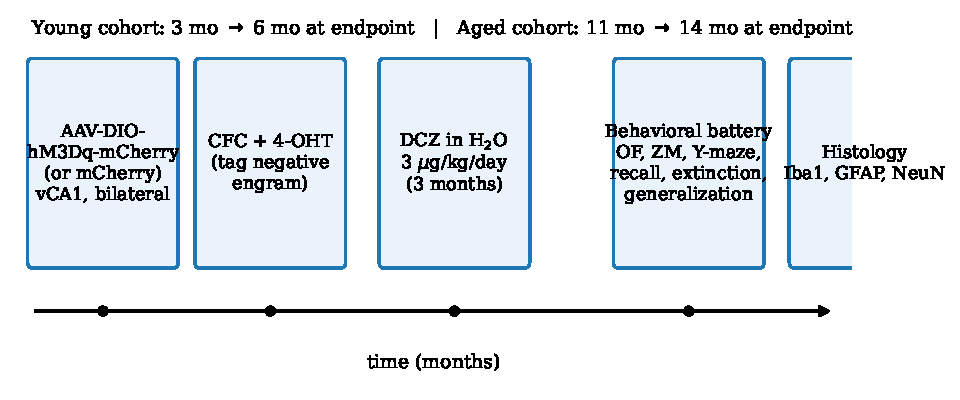
\includegraphics[width=0.95\textwidth]{figures/fig1_design_schematic.pdf}
\caption{\textbf{Experimental design.} TRAP2 mice received bilateral vCA1 injection of AAV9-DIO-Flex-hM3Dq-mCherry or AAV9-DIO-Flex-mCherry (300\,nL total). Two weeks later, contextual fear conditioning (four 1.5\,mA foot shocks in context A) was followed by $40\,\mathrm{mg\,kg^{-1}}$ i.p.\ 4-OHT to tag the negative engram. Chronic activation used DCZ in home-cage drinking water ($3\,\mu\mathrm{g\,kg^{-1}\,day^{-1}}$, refreshed every 5 days) for 3 months. Young and aged cohorts (3\,mo and 11\,mo at surgery) reached 6\,mo and 14\,mo at endpoint. Endpoint assays: open field, zero maze, Y-maze, remote recall, extinction, and generalization, followed by histology (Iba1, GFAP, NeuN).}
\label{fig:design}
\end{figure}

\begin{figure}[htbp]
\centering
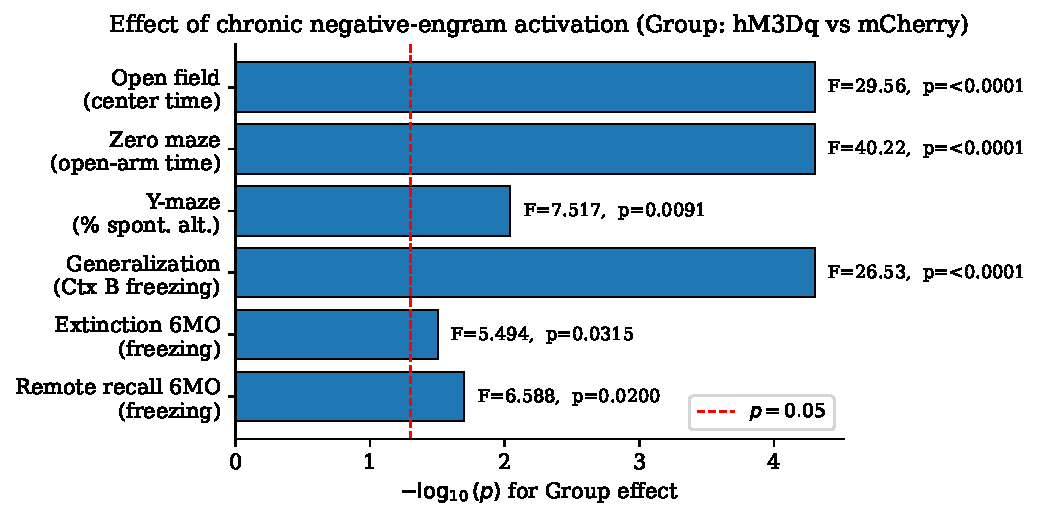
\includegraphics[width=0.85\textwidth]{figures/fig2_behavior_summary.pdf}
\caption{\textbf{Behavioral outcomes across assays, pooled across age.} $-\log_{10}(p)$ of the two-way ANOVA Group main effect (hM3Dq vs mCherry), with $F$ and $p$ values annotated. Significant Group effects for open-field center time ($F(1,33)=29.56$, $p<0.0001$), zero-maze open-arm time ($F(1,38)=40.22$, $p<0.0001$), Y-maze spontaneous alternation ($F(1,40)=7.517$, $p=0.0091$), Context\,B generalization freezing ($F(1,41)=26.53$, $p<0.0001$), 6-month extinction ($F(1,17)=5.494$, $p=0.0315$), and 6-month remote recall ($F(1,17)=6.588$, $p=0.0200$).}
\label{fig:behavior}
\end{figure}

\begin{figure}[htbp]
\centering
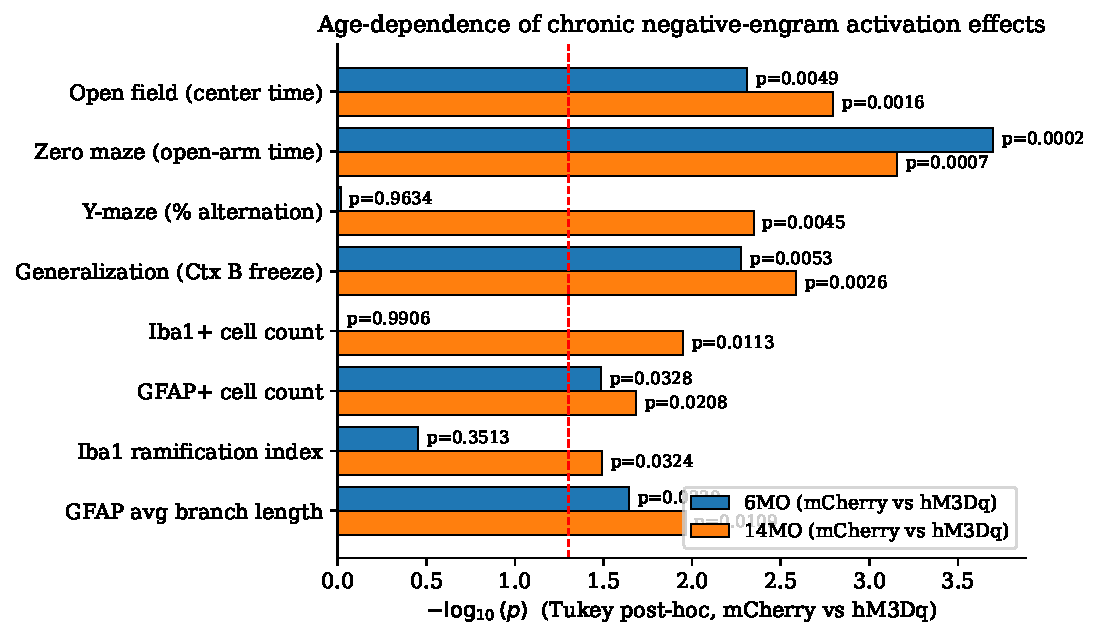
\includegraphics[width=0.9\textwidth]{figures/fig3_age_by_group_tukey.pdf}
\caption{\textbf{Age-by-group Tukey post-hoc comparisons.} Per-age Tukey $p$-values for hM3Dq vs age-matched mCherry, plotted as $-\log_{10}(p)$. Anxiety and generalization freezing reach significance at both ages; Y-maze alternation is impaired only at 14\,mo (6MO $p=0.9634$; 14MO $p=0.0045$). Iba1$^{+}$ count increases only at 14\,mo ($p=0.0113$; 6MO $p=0.9906$); GFAP$^{+}$ count increases at both ages (6MO $p=0.0328$; 14MO $p=0.0208$).}
\label{fig:age_by_group}
\end{figure}

\begin{figure}[htbp]
\centering
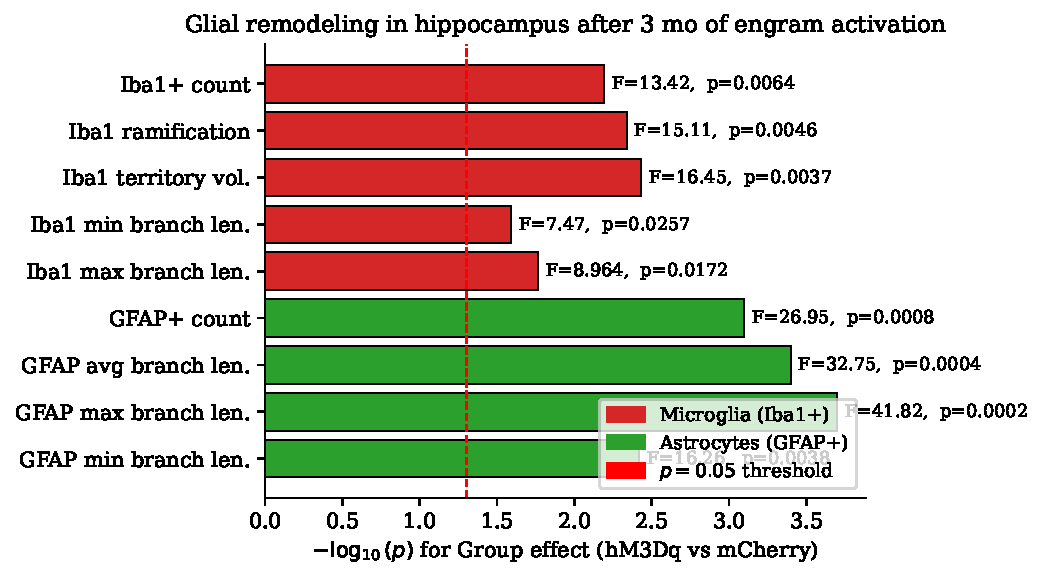
\includegraphics[width=0.85\textwidth]{figures/fig4_glia_summary.pdf}
\caption{\textbf{Glial remodeling in hippocampus after 3 months of chronic negative-engram activation.} Two-way ANOVA Group $F$-statistics and $p$-values for Iba1$^{+}$ and GFAP$^{+}$ metrics: Iba1$^{+}$ count ($F(1,8)=13.42$, $p=0.0064$), ramification ($p=0.0046$), territory volume ($p=0.0037$), min.\ ($p=0.0257$) and max.\ branch length ($p=0.0172$); GFAP$^{+}$ count ($F(1,8)=26.95$, $p=0.0008$), avg.\ ($p=0.0004$) and max.\ branch length ($p=0.0002$), and min.\ branch length ($p=0.0038$).}
\label{fig:glia}
\end{figure}

\begin{figure}[htbp]
\centering
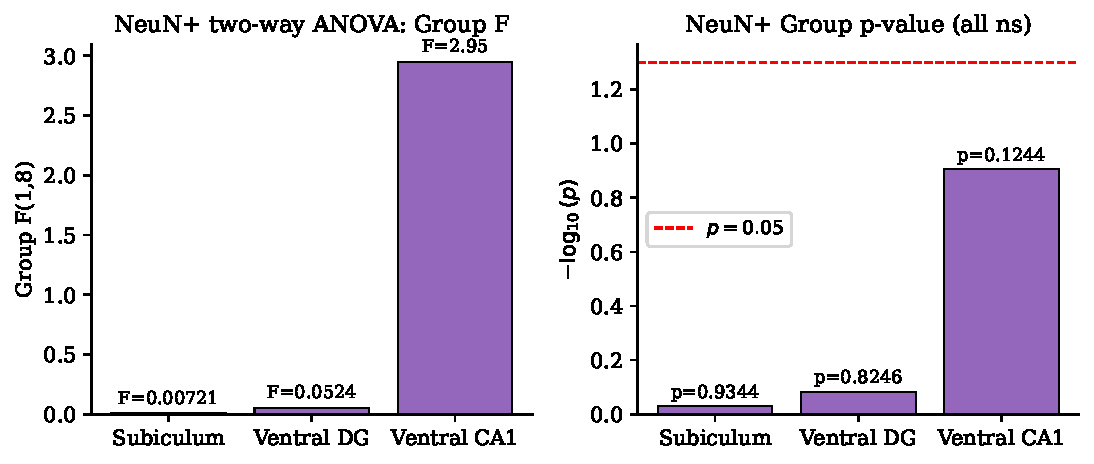
\includegraphics[width=0.85\textwidth]{figures/fig5_neun_safety.pdf}
\caption{\textbf{Chronic activation does not reduce NeuN$^{+}$ counts.} Two-way ANOVA Group $F$-statistics (left) and $-\log_{10}(p)$ (right) for NeuN$^{+}$ counts in subiculum ($F(1,8)=0.00721$, $p=0.9344$), ventral dentate gyrus ($F(1,8)=0.0524$, $p=0.8246$), and ventral CA1 ($F(1,8)=2.947$, $p=0.1244$).}
\label{fig:neun}
\end{figure}

\begin{figure}[htbp]
\centering
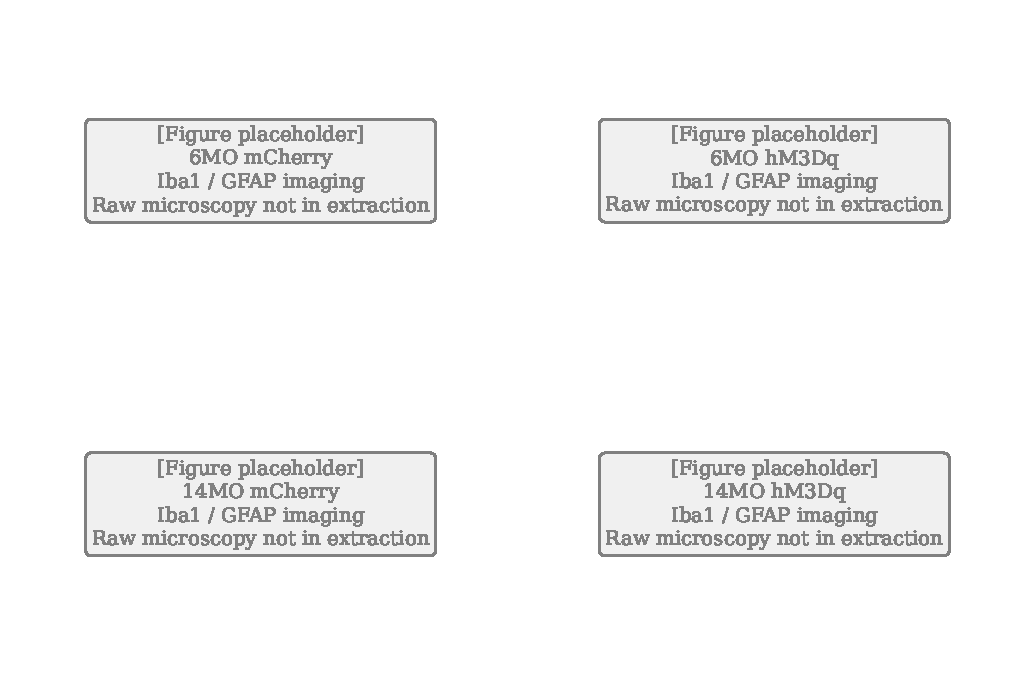
\includegraphics[width=0.8\textwidth]{figures/fig6_microscopy_placeholder.pdf}
\caption{\textbf{Representative Iba1$^{+}$ and GFAP$^{+}$ microscopy (placeholder).} Raw imaging panels for 6\,mo and 14\,mo mCherry and hM3Dq mice are shown schematically; corresponding 3DMorph-derived quantifications are in Figs.~\ref{fig:glia} and \ref{fig:age_by_group}.}
\label{fig:microscopy}
\end{figure}

% =====================================================================
\section{Discussion}

The central finding of this study is that three continuous months of chemogenetic reactivation of a single, vCA1-tagged negative memory engram is sufficient to induce a coherent constellation of behavioral and cellular abnormalities in mice, and that these abnormalities are partially but systematically age-dependent. At the level of summary statistics, the manipulation produced large and unambiguous Group effects on anxiety (open field $F(1,33)=29.56$, zero maze $F(1,38)=40.22$; both $p<0.0001$), fear generalization (Context~B $F(1,41)=26.53$, $p<0.0001$), and astrocyte counts ($F(1,8)=26.95$, $p=0.0008$), complemented by age-specific effects on working memory (14MO Y-maze Tukey $p=0.0045$), extinction (6MO $p=0.0315$), and microglial expansion (14MO $p=0.0113$). Crucially, all of these changes occurred without loss of NeuN$^{+}$ neurons in subiculum, ventral dentate gyrus, or ventral CA1, and without disruption of weight gain. These data argue that the repeated engagement of an aversive memory ensemble is not merely a readout of stress but a mechanistically sufficient driver of stress-like pathology, and they provide a causal framework within which to interpret the epidemiological link between repetitive negative thinking and adverse brain outcomes \citep{marchant2020rnt}.

A striking feature of the results is the valence-specificity implied by the engram transcriptomics. Positive (male-to-female exposure) and negative (foot-shock) engrams differed in their GSEA-ranked gene programs, with negative engrams enriched for pro-inflammatory pathways. This molecular bias meshes with the glial phenotype we observe after chronic reactivation: expanded GFAP$^{+}$ astrocyte counts at both ages, expanded Iba1$^{+}$ microglia at 14 months, and morphology changes that are consistent with reactive states in both cell types \citep{york2018threedmorph}. Our work thus offers a plausible causal chain from a molecularly distinct memory representation, through its chronic reactivation, to glial remodeling that mirrors the cellular signatures of chronic stress.

The age-dependence of the behavioral phenotypes is equally informative. Chronic activation impaired spatial working memory only in aged mice, while it impaired fear extinction and elevated remote recall only in young mice, even though both cohorts received an identical manipulation. This dissociation aligns with the glucocorticoid cascade framework, in which aged hippocampi are more susceptible to the cognitive consequences of sustained hippocampal drive \citep{sapolsky1986glucocorticoid}, and with the known decline of hippocampal neurogenesis with age that may narrow the brain's capacity for fear-memory updating \citep{klempin2007neurogenesis}. Conversely, the greater extinction impairment in young mice is consistent with an intact but hyper-engaged fear system, and can be interpreted within the hippocampus-amygdala-medial-prefrontal framework for fear learning and generalization \citep{maren2013contextual,tovote2015circuits}. Together, these results caution against treating "chronic stress" as a monolithic phenotype: the same causal manipulation produces qualitatively different deficits across the lifespan, and translational interpretation of preclinical data should take this age-by-phenotype interaction seriously.

Our findings complement prior engram literature in an important way. Most previous engram-manipulation studies operate on acute or short timescales, demonstrating that reactivation of a tagged ensemble is sufficient for episodic memory expression \citep{liu2012engram,redondo2014valence,ramirez2015positive,josselyn2020engram}. By extending the reactivation window to three continuous months and by using a low-dose, drinking-water-based DCZ protocol that mimics sustained dysregulation rather than acute, high-amplitude stimulation, we show that the biological consequences of engram reactivation are not limited to episodic recall: they include anxiety-like traits, context-generalization, and glial changes that persist in the absence of an immediate reactivating stimulus \citep{nagai2020dcz,roth2016dreadds,denardo2019temporal}. The magnitude of the Group effects we report (e.g., open-field Group $F(1,33)=29.56$, zero-maze Group $F(1,38)=40.22$, generalization Group $F(1,41)=26.53$, all $p<0.0001$) indicates that these effects are robust rather than marginal, supporting their interpretation as a genuine cellular-and-behavioral phenotype of chronic negative-engram activation.

Several limitations deserve explicit mention. First, TRAP2 and alternative Dox-based tagging systems capture different fractions of CA1 pyramidal cells (5--18\% vs.\ 20--40\% in prior reports), which means our "engram" is a subset rather than the totality of active neurons during conditioning, and direct comparison across tagging systems is non-trivial. Second, DCZ has rapid pharmacokinetics---peaking 5--10 min after IP injection and declining to baseline around 2 h---so although our home-cage drinking-water regimen is designed to produce sustained low-level activation tied to the animal's natural drinking schedule, the effective activation profile is likely a series of frequent, brief pulses tiled across the day rather than a perfect tonic drive \citep{nagai2020dcz}. This distinction matters for interpreting the phenotypes as models of sustained, rumination-like reactivation versus intermittent stressor-like engagement. Third, DREADD toxicity has been reported at high AAV titers in hippocampus; our low-dose, long-duration protocol together with the absence of NeuN$^{+}$ loss argues against overt toxicity, but subtle excitotoxic effects cannot be fully excluded. Fourth, we have not separately quantified excitatory versus inhibitory markers, leaving open the question of whether the effects are mediated by shifts in excitation-inhibition balance; this is an important target for future work. Finally, we did not include a Month~0 body-weight measurement, so a transient early drop in weight cannot be ruled out.

Looking forward, several extensions are suggested by this work. Projection-specific manipulation of vCA1 outputs to basolateral amygdala, nucleus accumbens, and prefrontal cortex \citep{ciocchi2015vca1} would allow the anxiety, generalization, and working-memory phenotypes to be assigned to specific downstream circuits. Longitudinal in vivo imaging of microglia and astrocytes during the three-month protocol would clarify whether glial remodeling precedes, tracks, or follows the behavioral changes. Pharmacological rescue experiments targeting pro-inflammatory pathways---whose signature we detect in negative engram transcriptomes---would test whether they are mechanistically required for the downstream behavioral phenotype. More broadly, the framework developed here, in which chronic engram reactivation is used as a causal model of rumination-like states, offers a new handle on the neurobiology of negatively valenced repetitive thought and its long-term brain consequences, including those previously linked to early neurodegenerative risk \citep{marchant2020rnt}.

% =====================================================================
\bibliographystyle{unsrtnat}
\bibliography{references}

\end{document}
